% \special{dvipdfmx:config z 0}
\documentclass[UTF8,a4paper,AutoFakeBold,AutoFakeSlant]{article}
\usepackage[a4paper,left=2.8cm,right=2.6cm,top=3.7cm,bottom=3.5cm]{geometry}
\usepackage{CTEX}
% \usepackage{xeCJK}
\usepackage{graphicx}
\usepackage{pythonhighlight}
\usepackage[mathscr]{eucal}
\usepackage{mathrsfs}
\usepackage{booktabs}
\usepackage{capt-of} 
\usepackage{hyperref} 
\usepackage{abstract}
\usepackage{amsmath}
\usepackage{listings}
\usepackage{color}
\usepackage{caption}
\usepackage{subfigure}
\usepackage{enumerate}
\usepackage{amsfonts} 
\usepackage{CJK,CJKnumb}
\usepackage{float}
% \usepackage{gbt7714}
\usepackage{framed}
\usepackage{multirow}


\newcommand{\song}{\CJKfamily{song}}    % 宋体   (Windows自带simsun.ttf)
\newcommand{\fs}{\CJKfamily{fs}}        % 仿宋体 (Windows自带simfs.ttf)
\newcommand{\kai}{\CJKfamily{kai}}      % 楷体   (Windows自带simkai.ttf)
\newcommand{\hei}{\CJKfamily{hei}}      % 黑体   (Windows自带simhei.ttf)
\newcommand{\li}{\CJKfamily{li}}        % 隶书   (Windows自带simli.ttf) 
\newcommand{\ssong}{\CJKfamily{STSong}}

\xeCJKsetup{SlantFactor = 0.3}
% \xeCJKsetup{SlantFactor = -0.7}
\setCJKmainfont[BoldFont=simhei.ttf, SlantedFont=simkai.ttf]{simsun.ttc}



% -- 中文字体 --
%\setCJKmainfont{Microsoft YaHei}  % 微软雅黑
%\setCJKmainfont{YouYuan}  % 幼圆
%\setCJKmainfont{NSimSun}  % 新宋体
%\setCJKmainfont{KaiTi}    % 楷体
% \setCJKmainfont{SimSun}   % 宋体
%\setCJKmainfont{SimHei}   % 黑体
% \setCJKfamilyfont{hwsong}{STSong}
 
% -- 英文字体 --
% \setmainfont{Times New Roman}
% \setmainfont{DejaVu Sans}
% \setmainfont{Latin Modern Mono}
% \setmainfont{Consolas}
% \setmainfont{Courier New}


\usepackage{xcolor}  	%高亮使用的颜色
\definecolor{commentcolor}{RGB}{85,139,78}
\definecolor{stringcolor}{RGB}{206,145,108}
\definecolor{keywordcolor}{RGB}{34,34,250}
\definecolor{backcolor}{RGB}{220,220,220}

\usepackage{accsupp}	
\newcommand{\emptyaccsupp}[1]{\BeginAccSupp{ActualText={}}#1\EndAccSupp{}}

\usepackage{listings}
\lstset{						%高亮代码设置
	language=python, 					%Python语法高亮
	linewidth=0.95\linewidth,      		%列表list宽度
	%basicstyle=\ttfamily,				%tt无法显示空格
	commentstyle=\color{commentcolor},	%注释颜色
	keywordstyle=\color{keywordcolor},	%关键词颜色
	stringstyle=\color{stringcolor},	%字符串颜色
	%showspaces=true,					%显示空格
	numbers=left,						%行数显示在左侧
	numberstyle=\tiny\emptyaccsupp,		%行数数字格式
	numbersep=5pt,						%数字间隔
	frame=single,						%加框
	framerule=0.1pt,						%划线
	escapeinside=@@,					%逃逸标志
	emptylines=1,						%
	xleftmargin=3em,					%list左边距
	backgroundcolor=\color{backcolor},	%列表背景色
	tabsize=4,							%制表符长度为4个字符
	% gobble=4							%忽略每行代码前4个字符
}




\renewcommand{\abstractname}{}    % clear the title
\renewcommand{\absnamepos}{empty}
%去除摘要两边缩进
\makeatletter
  \renewenvironment{abstract}{%
      \if@twocolumn
        \subsection*{\abstractname}%
      \else
        \small
        \begin{center}%
          {\bfseries \abstractname\vspace{-.5em}\vspace{\z@}}%
        \end{center}%
      \fi}
      {}
  \makeatother
  \lstset{
    language=Matlab,
    keywords={break,case,catch,continue,else,elseif,end,for,function,
       global,if,otherwise,persistent,return,switch,try,while},
    basicstyle=\ttfamily,
    keywordstyle=\color{blue}\bfseries,
    commentstyle=\color{dkgreen},
    stringstyle=\color{dkpurple},
    backgroundcolor=\color{white},
    tabsize=4,
    showspaces=false,
    showstringspaces=false
 }

\title{\textbf{\textsf{{\textsf{LB1} \heiti{机器学习概论}}}}} 
\author{\ssong PB19151769~~~~~~马宇骁}
\date{}

% 去掉红框
\hypersetup{
colorlinks=true,
linkcolor=black
}

\begin{document}



\maketitle

% \tableofcontents
% \newpage



\section{实验要求}

\subsection{Tasks}
In `​Logistic.py`, write your own Logistic Regression class Logistic.py

In `Load.ipynb`
\begin{enumerate}
  \item Deal with NULL rows, you can either choose to drop them or replace them with mean or other value
  \item Encode categorical features
  \item Split the dataset into X\_train, X\_test, y\_train, y\_test, also you can then use normalization or any other methods you want
  \item Train your model and plot the loss curve of training
  \item Compare the accuracy(or other metrics you want) of test data with different parameters you train with, i.e. learning rate, regularization methods and parameters .etc
\end{enumerate}


\subsection{Requirements}
\begin{itemize}
  \item Do not use sklearn or other machine learning library, you are only permitted with numpy, pandas, matplotlib, and Standard Library, you are required to write this project from scratch.
  \item You are allowed to discuss with other students, but you are not allowed to plagiarize the code*, we will use automatic system to determine the similarity of your programs, once detected, both of you will get zero mark for this project.
\end{itemize}



\section{实验原理}

实验主要运用Logistic Regression的知识进行分类回归和预测,在建立回归的时候需要理解梯度下降法并注意收敛条件。


\subsection{数据转换}
\subsubsection{类型转换}
机器学习模型需要的数据是数字型的,因为只有数字类型才能进行计算。因此,对于各种特殊的特征值,我们都需要对其进行相应的编码,也是量化的过程。
因此,对于实验数据集,做出两种不同的数据类型转换方式:
\begin{enumerate}
  \item Label encoding
  
  用标签进行编码的意思,即我们给特征变量自定义数字标签,量化特征。此数据集中将Gender,	Married,	Dependents,	Education,	Self\_Employed和Loan\_Status做该转换
  \item One-hot encoding
  
  独热编码(哑变量)定类型数据。将原始特征变量转换成以原始特征值分类的多维度的变量,并用是否(0,1)这种方式的新特征值替代和量化。此数据集中将Property\_Area的三类数据分离出来。
\end{enumerate}

\subsubsection{归一化}
正则化的方式有很多,例如:Sigmiod,arctan,log函数转换,z-score 标准化,min-max标准化等。由于该数据集需要转换的数据
都是非负数据,且使用arctan使得数据接近1区分很小,故考虑使用min-max标准化对表格中的4类数据转化。
\begin{itemize}
  \item min-max标准化(Min-max normalization)
\end{itemize}
\begin{equation*}
  x^* = \frac{x-min}{max-min}
\end{equation*}


\subsection{Logistic Regression逻辑回归}
Logistic 回归是一种统计方法,用于根据先前的观察结果预测因变量的结果。它是一种回归分析,是解决二元分类问题的常用算法。
逻辑回归也称为二项逻辑回归或二元逻辑回归。如果响应变量有两个以上类别,则称为多项逻辑回归。

逻辑回归的表示方式类似于使用直线方程定义线性回归的方式。与线性回归的显着区别是输出将是二进制值(0 或 1)而不是数值。

\begin{equation}
  h_{\theta}(x)=g\left(\theta^{T} x\right)=\frac{1}{1+e^{-\theta^{T} x}}
  \label{eq1}
\end{equation}
其中,$\theta_{0}+\theta_{1} x_{1}+, \ldots,+\theta_{n} x_{n}=\sum_{i=1}^{n} \theta_{i} x_{i}=\theta^{T} x$.

应用逻辑回归来预测分类因变量。换句话说,当预测是分类的时使用它,例如,是或否,真或假,0 或 1。逻辑回归的预测概率或输出可以是其中之一,没有中间立场。

对于预测变量,它们可以是以下任何类别的一部分:

\begin{itemize}
  \item 连续数据:可以在无限尺度上测量的数据。它可以取两个数字之间的任何值。例如以磅为单位的重量或以华氏度为单位的温度。
  \item 离散的名义数据:适合命名类别的数据。一个简单的例子是头发颜色:金色、黑色或棕色。
  \item 离散、有序的数据:符合某种规模顺序的数据。例如,以 1 到 5 的等级说明您对产品或服务的满意程度。
\end{itemize}

逻辑回归分析对于预测事件的可能性很有价值。它有助于确定任何两个类之间的概率。

因此,此次实验使用逻辑回归对Loan\_Status进行回归,预测判断这个人是否可以贷款。


\subsection{损失}

对数似然函数为:
\begin{equation*}
  l(\theta)=\log L(\theta)=\sum_{i=1}^{m}\left(y_{i} \log h_{\theta}\left(x_{i}\right)+\left(1-y_{i}\right) \log \left(1-h_{\theta}\left(x_{i}\right)\right)\right)
\end{equation*}
记 $D$ 为对数似然去掉符号的函数,则定义平均损失为:
\begin{equation*}
  J(\theta)=\frac{1}{n} \sum_{i=1}^{n} D\left(h_{\theta}\left(x_{i}\right), y_{i}\right)
\end{equation*}


\subsection{梯度下降}
\subsubsection{原理与实现}
循环执行以下 3 步骤:
\begin{enumerate}
  \item 环顾周围找到最陡的一段路
  \item 在最陡的一段路上走一段距离
  \item 重复以上步骤直到山底
\end{enumerate}

对一个函数应用梯度下降法,就是为了最快地求出函数的全局最小值或者局部最小值;再对应到机器学习问题上,梯度下降法就是为了尽快求出模型代价函数最小值,进而得到模型参数;

所以梯度下降法要解决的问题就是:以最快速度求函数最小值。
\begin{equation*}
  \theta_{j}=\theta_{j}-\alpha \frac{\partial}{\partial \theta_{j}} J(\theta)
\end{equation*}
计算梯度就是代价函数对 $\theta_i$ 进行复合求导:
\begin{equation*}
  J\left(\theta_{0}, \theta_{1}\right)^{\prime} = 2 * \frac{1}{2 m} \sum_{i = 1}^{m}\left(h_{\theta}\left(x_{i}\right)-y^{(i)}\right) * h_{\theta}\left(x_{i}\right)^{\prime}
\end{equation*}
\begin{equation*}
  h_{\theta}\left(x_{i}\right)^{\prime} = \left(\theta_{0} x_{0}+\theta_{1} x_{1}\right)^{\prime} = x_{i}
\end{equation*}

对于此时的逻辑回归有:
\begin{equation*}
  \begin{aligned}
    \frac{\partial }{\partial {\theta_j}} J(\theta) & = -\frac{1}{m} \sum_{i = 1}^{m}\left(y_{i} \frac{1}{h_{\theta}\left(x_{i}\right)} \frac{\partial }{\partial {\theta_j}} h_{\theta}\left(x_{i}\right)-\left(1-\mathrm{y}_{\mathrm{i}}\right) \frac{1}{1-h_{\theta}\left(x_{i}\right)} \frac{\partial }{\partial {\theta_j}} h_{\theta}\left(x_{i}\right)\right) \\ 
    & = -\frac{1}{m} \sum_{i  = 1}^{m}\left(y_{i} \frac{1}{g\left(\theta^{\mathrm{T}} x_{i}\right)}-\left(1-\mathrm{y}_{\mathrm{i}}\right) \frac{1}{1-g\left(\theta^{\mathrm{T}} x_{i}\right)}\right) \frac{\partial }{\partial {\theta_j}} g\left(\theta^{\mathrm{T}} x_{i}\right)\\
    &=-\frac{1}{m} \sum_{i=1}^{m}\left(y_{i} \frac{1}{g\left(\theta^{\mathrm{T}} x_{i}\right)}-\left(1-\mathrm{y}_{\mathrm{i}}\right) \frac{1}{1-g\left(\theta^{\mathrm{T}} x_{i}\right)}\right) g\left(\theta^{\mathrm{T}} x_{i}\right)\left(1-g\left(\theta^{\mathrm{T}} x_{i}\right)\right) \frac{\partial }{\partial {\theta_j}} \theta^{\mathrm{T}} x_{i} \\
    &=-\frac{1}{m} \sum_{i=1}^{m}\left(y_{i}\left(1-g\left(\theta^{\mathrm{T}} x_{i}\right)\right)-\left(1-\mathrm{y}_{\mathrm{i}}\right) g\left(\theta^{\mathrm{T}} x_{i}\right)\right) x_{i}^{j} \\
    &=-\frac{1}{m} \sum_{i=1}^{m}\left(y_{i}-g\left(\theta^{\mathrm{T}} x_{i}\right)\right) x_{i}^{j} \\
    &=\frac{1}{m} \sum_{i=1}^{m}\left(h_{\theta}\left(x_{i}\right)-y_{i}\right) x_{i}^{j}
    \end{aligned}
\end{equation*}

\subsubsection{收敛与停止}
有3种情况一个判断收敛或者哪怕没有收敛但也应该停止:
\begin{enumerate}
  \item 损失不再下降
  \item 迭代次数过多
  \item 梯度已经降到0
\end{enumerate}
否则学习可能无法停止。


\subsection{预测}
通过回归学习过程中得到的$\theta$ 的值带回式\ref{eq1}中,使用测试集计算得出的值如果大于0.5则为1,小于则为0.以此作为预测。



\section{实验实现}
具体代码见附件Loan.ipynb与Logis.py文件,
使用学习率为0.01时的学习过程记录如下:
\begin{python}
  第2000次
	Train Loss: 0.468 
用时0.078998秒
第4000次
	Train Loss: 0.466 
用时0.148096秒
第6000次
	Train Loss: 0.465 
用时0.217119秒
第8000次
	Train Loss: 0.465 
用时0.293116秒
第10000次
	Train Loss: 0.465 
用时0.366115秒
第12000次
	Train Loss: 0.465 
用时0.435113秒
第14000次
	Train Loss: 0.465 
用时0.506114秒
第16000次
	Train Loss: 0.465 
用时0.582115秒
第18000次
...
用时3.250627秒
第92000次
	Train Loss: 0.465 
用时3.321548秒
\end{python}
损失曲线绘制如图:
\begin{figure}[htbp]
  \centering
  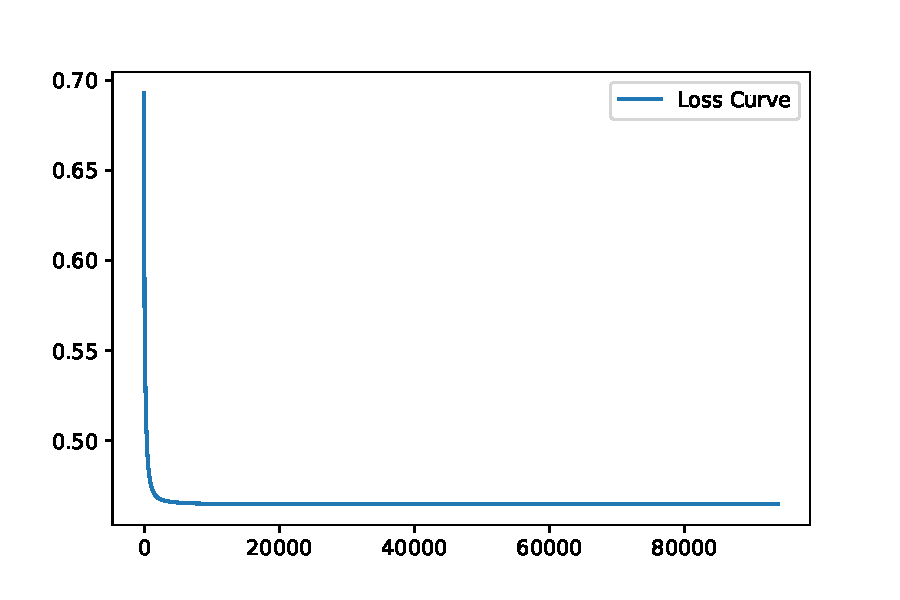
\includegraphics[scale=0.625]{loss.pdf}
  \caption{Loss Curve}
  \label{f1}
\end{figure}
可以发现,收敛速度很快。此时的预测准确率(随机打乱9:1的训练测试集比例):
\begin{quote}
  0.8541666666666666
\end{quote}
还是不错的。

经过尝试其他的学习率如0.1,可以发现收敛速度更快(有运气的成分),但由于集合的原因此时看不出预测准确率的很大区别。






















% \bibliographystyle{gbt7714-numerical}
% % \bibliographystyle{7714-author-year}
% \bibliographystyle{ieeetr}
% \bibliography{bibl}

\end{document}